% !TEX encoding = UTF-8 Unicode

\Chapter{Implementáció C++ és OpenCV segítségével}
\Section{OpenCV bemutatása}

Az OpenCV (Open Source Computer Vision Library) egy nyílt forráskódú számítógépes látás és gépi tanulási szoftverkönyvtár. Az OpenCV-t azért hozták létre, hogy közös infrastruktúrát biztosítson a számítógépes megjelenítési alkalmazások számára, és felgyorsítsa a gépi érzékelés használatát a kereskedelmi termékekben. BSD licenc alatt került kiadásra, ezért ingyenes mind tudományos, mind kereskedelmi célokra. C ++, Python és Java interfészekkel rendelkezik, és támogatja a Windows, Linux, Mac OS, iOS és Android rendszereket. Az OpenCV-et a számítási hatékonyságra tervezték, és nagy hangsúlyt fektetett a valós idejű alkalmazásokra. Az optimalizált C / C ++-ban írt, a könyvtár kihasználhatja a többmagos feldolgozást is. Az OpenCL használatával kihasználhatja az alapul szolgáló heterogén számítási platform hardveres gyorsítását.
\\

\noindent A könyvtár több mint 2500 optimalizált algoritmussal rendelkezik, amely magába foglalja mind a klasszikus, mind a legmodernebb számítógépes látásmódot és a gépi tanulási algoritmusokat. Ezek az algoritmusok felismerhetik az arcokat, felismerhetik az objektumokat, osztályozhatják az emberi cselekvéseket a videókban, nyomon követhetik a mozgásokat, követhetik a mozgó objektumokat, eltávolíthatja a vörös szemeket a vakuval készített képekből, követheti a szemmozgásokat, felismerheti a tájat stb. 
\\
%https://opencv.org
\Section{Beépített művészi jellegű OpenCV-s szűrők}
Az OpenCV könyvtár rendelkezik saját bepített, nem fotorealisztikus szűrőkkel, amelyeknél csak a bemeneti képet, valamint néhány paramétert kell megadnunk a függvénynek és ő elkészíti nekünk a filterezett képet. Négy ilyen beépített függvény található az OpenCV-ben, Edge Preserving filter, Detail Enhancing filter, Pencil sketch filter és a Stylization filter. Ezek C++ implementációját szeretném bemutatni.
\SubSection{Edge Preserving filter}
Az első ilyen szűrő az Edge Preversing filter, ami az éleket megörzi de a hátteret elmossa. 
\begin{cpp}
edgePreservingFilter(Mat src, Mat dst, int flags=1, 
			float sigma_s=60, float sigma_r=0.4f);
\end{cpp}
ahol, \textbf{src} a bemeneti kép, amit szertnénk átalakítani,\\
\indent \textbf{dst} a filterrel ellátot kép, \\
\indent \textbf{flags} maga az él kiemelő filter melynek két paramétere lehet, \textbf{RECURS\_FILTER} (rekurív szűrő) aminek az értéke 1 vagy \textbf{NORMCONV\_FILTER} (normalizált konvolúció) aminek az értéke 2.  A futási sebességtől függ melyik paramétert alkalmazzuk, ha gyorsabb sebességet akarounk elérni akkor a rekurzív filtert alkamazzuk, ha viszont nem számít a sebesség akkor a  normalizált konvolúciót mert az szebben kiemeli az éleket.\\
\indent \textbf{sigma\_s} egy skála 0 és 200 között, Sigma\_spatial a simítás mértékét határozzuk meg, \\
\indent \textbf{sigma\_r} egy skála 0 és 1 között, Sigma\_range szabályozza, hogy a szomszédságon belül a különböző színek milyen mértékben átlagolódjanak.
\begin{figure}[ht]
\centering
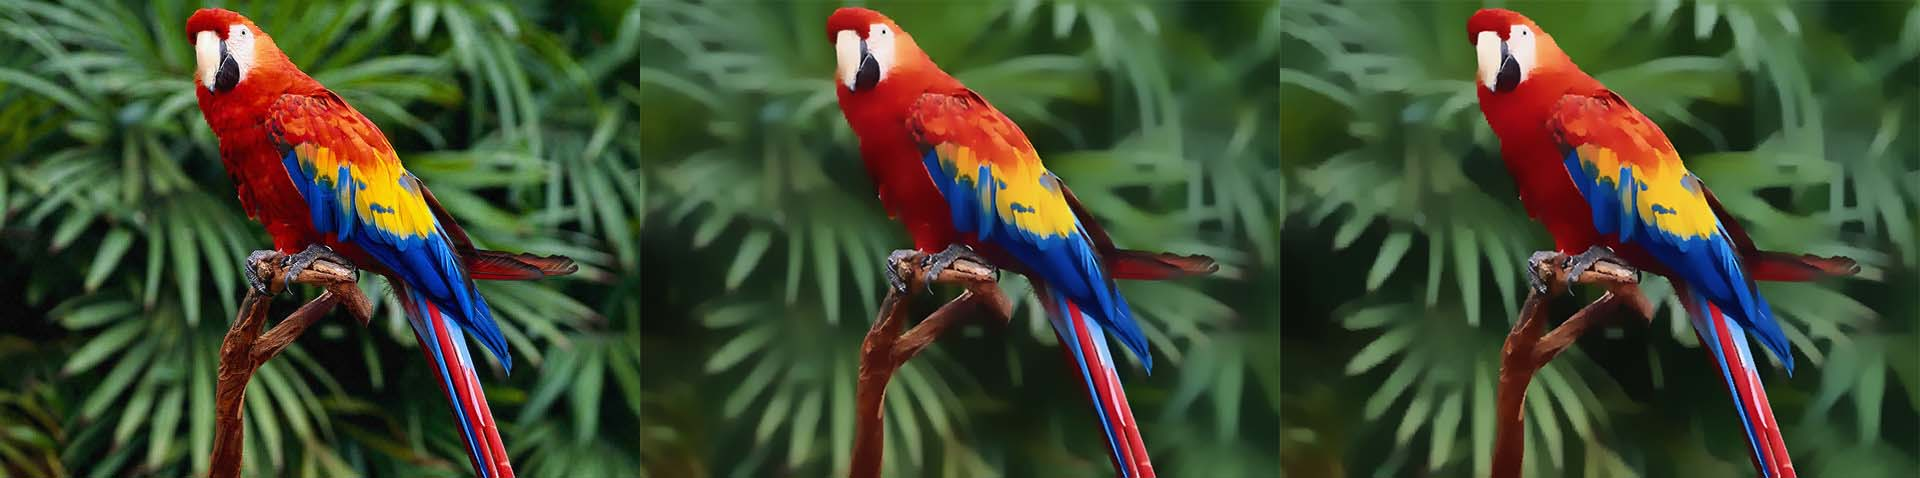
\epsfig{file=kepek/edgePreservingFilter.jpg,scale=0.45}
\caption{Eredeti kép, Rekurzív filter, Normalizált konvolúció} 
\label{fig: edgePreservingFilter}
\end{figure}
\newpage
\SubSection{Detail Enhancing filter}
A második ilyen szűrő a Detail Enhancing filter, ami a képet élesebbé teszi.
\begin{cpp}
detailEnhance(Mat src, Mat dst, float sigma_s=10, float sigma_r=0.15f);
\end{cpp}
A paraméterek megegyeznek az Edge Preserving filter paramétereivel. 
 \begin{figure}[ht]
\centering
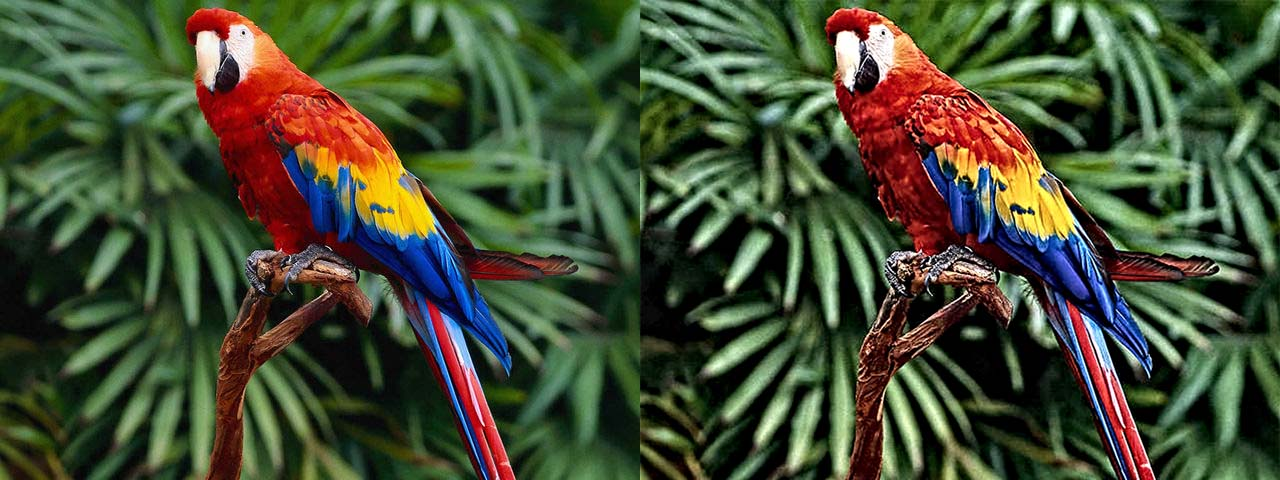
\epsfig{file=kepek/detailEnhance.jpg,scale=0.65}
\caption{Eredeti kép, Detail Enhancing filter eredménye} 
\label{fig:detailEnhance}
\end{figure}
\SubSection{Pencil sketch filter}
Ez a szűrő ceruza rajzot eredményez, két féle képet eredményez egy színes képet és egy szürkeárnyalatosat.
\begin{cpp}
pencilSketch(Mat src, Mat dst_gray, Mat dst_color, float sigma_s=60, 
		float sigma_r=0.07f, float shade_factor=0.02f);
\end{cpp}
A paraméterek megegyeznek az Edge Preserving szűrőével, de bővül egy paraméterrel.\\
\indent \textbf{shade\_factor}  ami egy 0 és 0,1 közötti érték, a kimeneti képintenzitás skálázása. Minél magasabb az érték, annál fényesebb az eredmény.
\begin{figure}[ht]
\centering
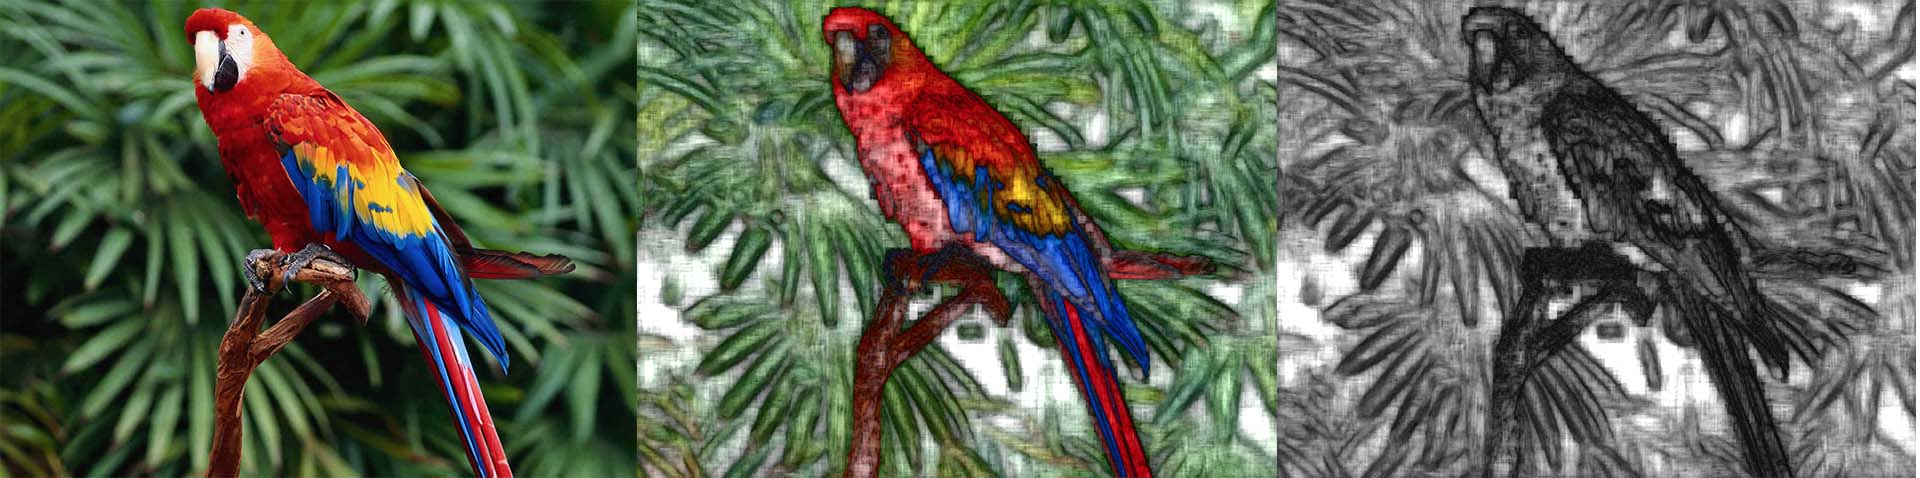
\epsfig{file=kepek/pencil_sketch_color_grey.jpg,scale=0.45}
\caption{Eredeti kép, Pencil sketch filter színes, Pencil sketch filter szűrkeárnyalatos} 
\label{fig: pencil_sketch_color_grey}
\end{figure}
\SubSection{Stylization filter}
A Stylization filter olyan kimeneti képet eredményez, aminek olyan hatása van mint ha vízfestékkel készítették volna.
\begin{cpp}
stylization(Mat src, Mat dst, float sigma_s=60, float sigma_r=0.45f);
\end{cpp}
A paraméterek megegyeznek az Edge Preserving filter paramétereivel. 
 \begin{figure}[ht]
\centering
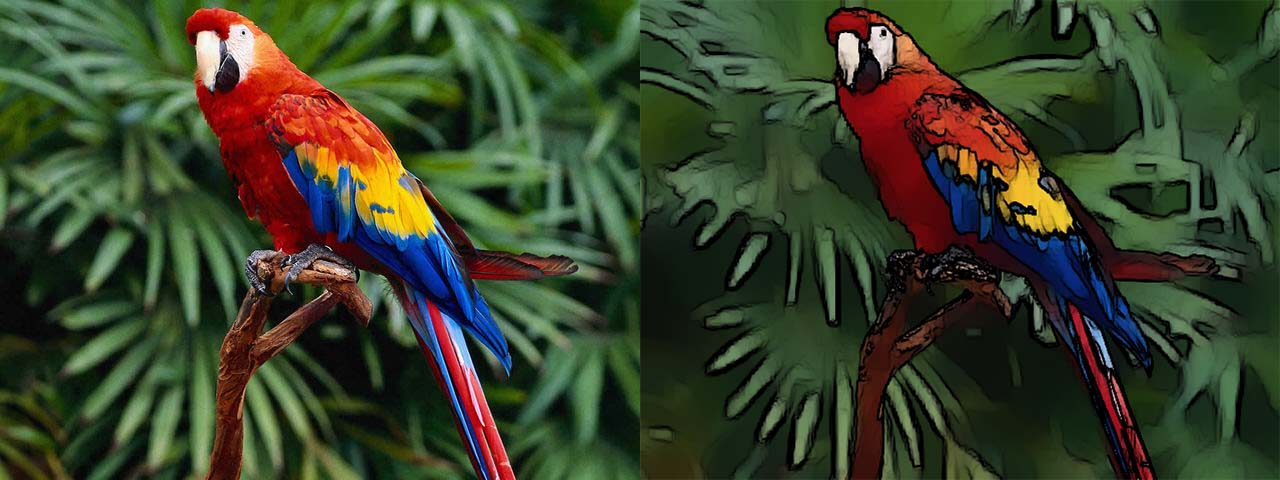
\epsfig{file=kepek/stylization.jpg,scale=0.65}
\caption{Eredeti kép, Stylization filter eredménye} 
\label{fig: stylization}
\end{figure}
%https://www.learnopencv.com/non-photorealistic-rendering-using-opencv-python-c/
\Section{Saját szűrők implementációja OpenCV és C++-al}
Ebben a fejezetben szeretném bemutatni a saját szűrőknek a C++ implementációját és a paramétereket amiket használtam hozzájuk. Itt képekkel nem fogok illusztrálni, mert azok a \textbf{4. fejezetben} megtalálhatóak. \\ Elsőként bemutatnám a kép betöltésének implementációját, amit minden szűrőn használtam.
\begin{cpp}
    Mat img = imread("image.jpg"); // bemeneti kep
    Mat dst ; //kimeneti kep
    //Ha valami nem stimmel a kep betoltesnel
    if ( img.empty() )
    {
        cout << "Error loading the image" << endl;
        return -1;
    }
\end{cpp} 
Ablak létrehozása :
\begin{cpp}
    namedWindow("Original image", 1);
    namedWindow("Image with filter", 1);
\end{cpp}
Ezután következik az a rész, amit a következő alfejezetekben fogok részletezni, hogy tulajdon képpen milyen lépésekből épül fel a filter. \\
Ezek után a kép megjelenítése:
\begin{cpp}
    imshow("Original imagel",img );
    imshow("Image with filter", dst);
\end{cpp}
És végezetül a waitKey funkció következik, amely a megadott milliszekundumban megjeleníti a képet. Mivel itt nem mozgó képről beszélünk igy az értéke 0.
 \begin{cpp}
    waitKey(0);
\end{cpp}
\SubSection{Cartoon-style filter}
Gauss piramisban lefelé lépünk kettőt.
\begin{cpp}
 for(int i=0; i < 2;i++){
    pyrDown( img, img);
    }
\end{cpp}
ahol, \\
\indent \textbf{img}: a bemeneti színes kép,\\
\indent \textbf{img}: a kimeneti kicsinyített színes kép.\\\\
Egymás után 7 szer hajtjuk végre a kétoldalú szűrőt.
\begin{cpp}
Mat img_res;
int d = 9;
double sigmaColor = 9.0;
double sigmaSpace = 7.0;
for(int i=0; i < 7;i++){
    bilateralFilter ( img, img_res, d, sigmaColor, sigmaSpace );
    }
\end{cpp}
ahol, \\
\indent \textbf{img}: a bemeneti színes kép,\\
\indent \textbf{img\_res}: a kimeneti kép kétoldalú szűrővel,\\
\indent \textbf{d}: a szűrés során használt minden egyes pixel szomszédság átmérője. Ha nem pozitív, akkor kiszámítható a sigmaSpace-ből,\\
\indent \textbf{sigmaColor}: szűri a szigmát a színtérben ,\\
\indent \textbf{sigmaSpace}: szűri a szigmát a koordinátatérben.\\ \\
Gauss piramisban felfelé lépünk kettőt, hogy visszanyerjük az eredeti kép méretet.
\begin{cpp}
 for(int i=0; i < 2;i++){
    pyrUp( img, img_res);
    }
\end{cpp}
ahol, \\
\indent \textbf{img}: a bemeneti színes kép,\\
\indent \textbf{img}: a kimeneti kicsinyített színes kép.\\\\
Kép konvertálása szürkeárnyalatossá. 
\begin{cpp}
cvtColor(img, srcGray, CV_BGR2GRAY);
\end{cpp}
ahol, \\
\indent \textbf{img}: a bemeneti színes kép,\\
\indent \textbf{srcGray}: a kimeneti szürkeárnyalatos kép,\\
\indent \textbf{CV\_BGR2GRAY}: színes kép szürkeárnyalatosra alakítására használatos paraméter.\\ \\
A következő lépésben a medián szűrőt implementáltam.
\begin{cpp}
int kernel_size = 7;
medianBlur(srcGray, median, kernel_size );
\end{cpp}
ahol, \\
\indent \textbf{srcGray}: a bemeneti szürkeárnyalatos kép,\\
\indent \textbf{median}: a kimeneti medián szűrővel ellátott kép,\\
\indent \textbf{kernel\_size}: a kernel mérete, itt ebben az esetben egy $7 x 7$-es mátrix. Ami már nem csak a zaj kiszűrését eredményezi, hanem már cartoon jellegűre mossa a képet.\\ \\
Adaptív küszöbölés implementációja.
\begin{cpp}
Mat img_edge;
double maxValue = 255;
int blockSize = 9;
double C = 2); 
adaptiveThreshold(median,img_edge, maxValue, ADAPTIVE_THRESH_MEAN_C,
		THRESH_BINARY,blockSize,C); 
\end{cpp}
ahol, \\
\indent \textbf{median}: a bemeneti medián szűrővel ellátott kép,\\
\indent \textbf{img\_edge}: a kimeneti éldetektálás eredménye,\\
\indent \textbf{maxValue}: nem zérus érték hozzárendelve azokhoz a képpontokhoz, amelyekhez a feltétel teljesül.\\ 
\indent \textbf{ADAPTIVE\_THRESH\_MEAN\_C}: adaptiv küszöbölés algoritmus,\\
\indent \textbf{THRESH\_BINARY}: a küszöbérték típusának THRESH\_BINARY vagy THRESH\_BINARY\_INV értékűnek kell lennie,\\
\indent \textbf{blockSize}: a pixel szomszédságának mérete, amelyet a pixel küszöbértékének kiszámítására használnak,\\
\indent \textbf{C}: a konstanst az átlagból vagy a súlyozott átlagból kell levonni, normális esetben pozitív, de lehet nulla vagy negatív is.\\\\
A maszk színesre konvertálása.
\begin{cpp}
cvtColor(img_edge, img_edge, CV_GRAY2RGB);
\end{cpp}
ahol, \\
\indent \textbf{img\_edge}: a bemeneti szürkeárnyalatos kép,\\
\indent \textbf{img\_edge}: a kimeneti színes kép,\\
\indent \textbf{CV\_GRAY2RGB}: szürkeárnyalatos kép színesre alakítására használatos paraméter.\\ \\
Az elmosott kép és a maszk egyesítése. 
\begin{cpp}
Mat img_cartoon;
bitwise_and(img_res,img_edge,img_cartoon);
\end{cpp}
ahol, \\
\indent \textbf{img\_res}: a bemeneti elmosott kép,\\
\indent \textbf{img\_edge}: a bemeneti élmaszk,\\
\indent \textbf{img\_cartoon}: kimeneti Cartoon-style filterezett kép.
\SubSection{Pencil sketch filter}
Első lépésként átkonvertáltam a képet színesről szűrkeárnyalatossá majd egy medián szűrést hajtottam végre. Ezt az előző szűrőnél már bemutattam így itt nem részletezném, ugyan azokat a paramétereket használtma itt is mint ott.\\
A következő lépésben egy Gauss simítást implementáltam. 
\begin{cpp}
Mat img_blur;
Size ksize = Size(21, 21);
double sigmaX = 0;
double sigmaY = 0;
GaussianBlur(median, img_blur, ksize, sigmaX, sigmaY);
\end{cpp}
ahol, \\
\indent \textbf{median}: a bemeneti medián szűrővel ellátott kép,\\
\indent \textbf{img\_blur}: a kimeneti Gauss szűrés eredménye,\\
\indent \textbf{ksize}: a kernel mérete, itt ebben az esetben egy $21 x 21$-es mátrix,\\
\indent \textbf{sigmaX}: a Gauss kernel standard elterese X iranyba,\\
\indent \textbf{sigmaY}: a Gauss kernel standard elterese Y iranyba.\\ \\
A medián és Gauss szűrő elosztása egymással.
\begin{cpp}
Mat img_blend;
double scale = 245;
divide(median, img_blur, img_blend, scale);   
\end{cpp}
ahol, \\
\indent \textbf{median}: a bemeneti medián szűrővel ellátott kép,\\
\indent \textbf{img\_blur}: a bemeneti Gauss szűrővel ellátott kép,\\
\indent \textbf{img\_blend}: a kimeneti kép a szűrők elosztásának eredménye,\\
\indent \textbf{scale}: a skalár tényező.\\ \\
Kontraszt széthúzás.
\begin{cpp}
double alpha=0; 
double beta=255;
normalize(img_blend, img_blend, alpha, beta, CV_MINMAX);
\end{cpp}
ahol,
\begin{itemize}
\item \texttt{img\_blend}: a két szűrő elosztásával kapott kép,
\item \texttt{img\_blend}: a kimeneti kontraszt széthúzással kapott kép,
\item \texttt{alpha}: normál érték a normálértékhez viszonyítva vagy az alsó tartomány határértéke esetén,
\item \texttt{beta}: első tartományhatár a tartomány normalizálása esetén,
\item \texttt{CV\_MINMAX}: választható maszk művelet.
\end{itemize}

A szürkeárnyalatos vászon összeszorzása a kontraszt széthúzott képpel.
\begin{cpp}
double scale = 1.0 / 256;
multiply(img_blend, canvas, img_blend, scale);
\end{cpp}
ahol, \\
\indent \textbf{img\_blend}: a bemeneti kontraszt széthúzással ellátott kép,\\
\indent \textbf{canvas}: a bemenet vászon képe,\\
\indent \textbf{img\_blend}: a kimeneti összeszorzott kép,\\
\indent \textbf{scale}: választható skálafaktor.\\\\
\SubSection{Cartoon filter}
Első lépésként itt mint az előző filtereknél, átkonvertáltam a képet színesről szűrkeárnyalatossá majd egy medián szűrést hajtottam végre.\\
Ezt egy Laplace éldetektálás követte.
\begin{cpp}
int kernel_size = 5;  
Laplacian(median, edges, CV_8U, kernel_size);
\end{cpp}
 ahol, \\
\indent \textbf{median}: a bemeneti median szűrővel ellátott kép,\\
\indent \textbf{edges}: az élekdetektálás eredménye,\\
\indent \textbf{CV\_8U}: unsigned 8bit / pixel - azaz egy pixel 0-255 értékű tartományban lehet,\\
\indent \textbf{kernel\_size}: a kernel mérete, itt ebben az esetben egy $5 x 5$-ös mátrix. Azt mutatja meg mekkora legyen a maszkon az él mérete.\\ \\
Végezetül a küszöbölés következett.
\begin{cpp}
double thresh = 90;
double maxval = 255;
threshold(edges, mask, thresh, maxval, THRESH_BINARY_INV);
\end{cpp}
 ahol, \\
\indent \textbf{edges}: a bemeneti kép az élekdetektálás eredménye,\\
\indent \textbf{mask}: a küszöbölés eredménye,\\
\indent \textbf{thresh}: küszöbérték,\\
\indent \textbf{maxval}: a THRESH\_BINARY és a THRESH\_BINARY\_INV küszöbérték típusokhoz használható maximális érték,\\
\indent \textbf{THRESH\_BINARY\_INV}:
 \[
 mask(x,y)=\left\{
 \begin{array}{ll}
 0 & \mbox{, ha edge$(x,y)$> thresh,}\\
 maxval & \mbox{, különben}
 \end{array}
 \right.
\]
\SubSection{Aquarelle-stlye filter}
Ez a filter két egyszerű lépésből áll az elős az egy átlagoló szűrő.
\begin{cpp}
Size ksize = Size(3, 3);
blur(img_rgb, img_rgb, ksize);
\end{cpp}
 ahol, \\
\indent \textbf{img\_rgb}: a bemeneti színes kép,\\
\indent \textbf{img\_rgb}: a kimeneti elmosott kép,\\
\indent \textbf{ksize}: a kernel mérete, itt ebben az esetben egy $3 x 3$-as mátrix. \\ \\
Mean shift szegmentáció.
\begin{cpp}
Mat img_shifted;
double sp = 15;
double sr = 50;
pyrMeanShiftFiltering(img_rgb,img_shifted, sp, sr);
\end{cpp}
 ahol, \\
\indent \textbf{img\_rgb}: a bemeneti színes kép,\\
\indent \textbf{img\_shifted}: a kimeneti elmosott kép,\\
\indent \textbf{sp}: a térbeli ablak sugara,\\
\indent \textbf{sr}: a színablak sugara.

%4-6 oldal


% Technikai jelleg rész